% CMP4509 Introduction to Deep Learning -- Term project report template
% Compiles with pdfLaTeX + BibTeX (Overleaf: upload this folder or the .zip).
%
% The grey boxes are guides describing what is expected in each section.
% Keep them visible while writing. Before submitting, hide them all by
% setting \showguidesfalse below. The supplied document structure is preserved.
\documentclass[11pt,a4paper]{article}

\usepackage[margin=2.5cm]{geometry}
\usepackage[T1]{fontenc}
\usepackage[utf8]{inputenc}
\usepackage{lmodern}
\usepackage{amsmath,amssymb,amsfonts}
\usepackage{graphicx}
\usepackage{placeins}
\usepackage{array}
\usepackage{microtype}
\usepackage{booktabs}
\usepackage{multirow}
\usepackage{caption}
\usepackage{subcaption}
\usepackage{xcolor}
\usepackage{enumitem}
\usepackage[round]{natbib}
\usepackage[colorlinks=true,linkcolor=blue,citecolor=blue,urlcolor=blue]{hyperref}

% ---------------------------------------------------------------------------
% Guide boxes
\newif\ifshowguides
\showguidesfalse   % instructional boxes disabled in the submitted version
\definecolor{guidebg}{gray}{0.93}
\definecolor{guideframe}{gray}{0.55}
\newcommand{\guide}[1]{%
  \ifshowguides
  \par\medskip\noindent
  \fcolorbox{guideframe}{guidebg}{%
    \begin{minipage}{\dimexpr\linewidth-2\fboxsep-2\fboxrule\relax}
      \small\textbf{Guide.}
      \begin{itemize}[leftmargin=1.2em,itemsep=1pt,topsep=2pt]
        #1
      \end{itemize}
    \end{minipage}}%
  \par\medskip
  \fi}
% ---------------------------------------------------------------------------

% Notation shortcuts (optional)
\newcommand{\R}{\mathbb{R}}
\newcommand{\E}{\mathbb{E}}
\newcommand{\vect}[1]{\mathbf{#1}}
\newcommand{\linf}{\ell_\infty}
\newcommand{\TODO}[1]{\textbf{[TO FILL: #1]}}

\title{Reproducing ``\textit{Towards Deep Learning Models Resistant to Adversarial Attacks}''\\[0.3em]
\large CMP4509 Introduction to Deep Learning --- Term Project Report}
\author{Muhammed Emir Baka\c{c}\\(2368574) \and
Mehmet Efe \c{C}ak\i r\\(2201123) \and
Sena Sa\u{g}d\i\c{c}\\(2201275)}
\date{October 25, 2026}
\hypersetup{
  pdftitle={MNIST Adversarial Training: A Scaled Reproduction of Madry et al.},
  pdfauthor={Muhammed Emir Bakac; Mehmet Efe Cakir; Sena Sagdic},
  pdfsubject={CMP4509 term project; empirical adversarial robustness},
  pdfkeywords={MNIST, adversarial training, PGD, reproducibility},
  unicode=true
}

\begin{document}
\maketitle

\begin{abstract}
We investigate the central claim of \citet{madry2018towards} that training against projected-gradient-descent (PGD) adversarial examples improves resistance to first-order attacks. We reproduce the method with a smaller, 215,370-parameter PyTorch convolutional neural network on MNIST and a free Google Colab T4 GPU. We compare standard training, 40-step PGD training from random initialization, and an additional curriculum using 10 PGD steps for three epochs followed by 40 steps for seven epochs. Across three random training seeds, standard training achieves $99.03\pm0.05\%$ clean accuracy but $0.00\pm0.00\%$ under a frozen $\linf$-bounded PGD attack ($\varepsilon=0.3$, 100 steps, five random restarts). Direct PGD40 training reaches $31.28\pm34.53\%$ under this attack; two of three selected checkpoints have only $11.35\%$ clean and attacked accuracy, consistent with the authors' reported training collapse. Curriculum training reaches $97.85\pm0.30\%$ clean and $88.13\pm0.87\%$ PGD accuracy. These findings support the adversarial-training claim in our restricted setting, while demonstrating optimization sensitivity to initialization and the importance of attack-strength and model-capacity qualifications.
\end{abstract}

\guide{
  \item One paragraph, written last.
  \item A reader should learn four things: which paper, which claim, in what setting, and the outcome.
  \item Give your main result as a number (e.g.\ accuracy, mean $\pm$ std), not as ``good'' or ``promising''.
}

\section{Introduction}
\label{sec:intro}
High classification accuracy on unmodified inputs is not sufficient to ensure reliability under intentional perturbations. An attacker can modify the pixels of an image within a small, explicitly bounded region while causing an otherwise accurate neural network to change its prediction. \citet{goodfellow2015explaining} presented gradient-based adversarial examples; \citet{madry2018towards} formulated defense as a robust optimization problem that treats attacking and training as the inner and outer stages of a single min--max objective.

\textbf{Tested claim.} Relative to training on clean MNIST images, training on high-loss examples generated by multi-step PGD can greatly improve accuracy against $\linf$-constrained gradient attacks. This is the central MNIST claim illustrated by Figure~3 and Table~1 of \citet{madry2018towards}; the authors report $89.3\%$ adversarial accuracy against a 100-step, 20-restart white-box PGD adversary for their larger trained network. Our principal comparison is standard training versus direct PGD40, with an exploratory PGD10$\rightarrow$PGD40 schedule prompted by failures in two direct-training seeds. Our report does \emph{not} claim to reproduce every numerical result or architectural detail of the original paper.

We use the same MNIST split, network, optimizer settings, seed set, and final test attack across methods, with the validation checkpoint-selection rules specified in Section~\ref{sec:setup}. We report three seeds for every final condition, including unsuccessful runs. Additional author-reported validation attacks probe whether PGD scores are optimistic; their raw logs are unavailable in the audited snapshot. The complete source code and the nine final test measurements are available through our public repository (see the \hyperref[sec:code]{Code section}).


\guide{
  \item Explain the problem the paper addresses and why it mattered at the time.
  \item State the claim you test in one or two precise sentences, and point to the exact figure, table or section of the paper it comes from.
  \item A testable claim names what is compared and what is expected, e.g.\ ``network A reaches lower training loss than network B at depth $L$''. ``The method works well'' is not a claim.
  \item Do not reproduce the paper's abstract.
}

\section{Background and Method}
\label{sec:method}
\subsection{From empirical risk to robust risk}
Consider an input image flattened into $x\in\R^{d}$ with $d=28\cdot28=784$, label $y\in\{0,\ldots,9\}$, trainable parameters $\theta\in\R^p$, and network logits $f_\theta(x)\in\R^{10}$. A minibatch is $\vect{X}\in\R^{B\times1\times28\times28}$, with $B=128$ during the main experiments, and the corresponding logits have shape $B\times10$. For a single example, cross entropy is
\begin{equation}
\mathcal{L}(\theta,x,y)=-\log\left(\frac{e^{f_\theta(x)_y}}{\sum_{k=0}^{9}e^{f_\theta(x)_k}}\right).
\label{eq:ce}
\end{equation}
The clean population risk is $R(\theta)=\E_{(x,y)\sim\mathcal{D}}[\mathcal{L}(\theta,x,y)]$. Given training samples $\{(x_i,y_i)\}_{i=1}^{n}$, empirical risk minimization instead minimizes
\begin{equation}
\widehat R_n(\theta)=\frac{1}{n}\sum_{i=1}^{n}\mathcal{L}(\theta,x_i,y_i).
\label{eq:erm}
\end{equation}
This empirical objective penalizes errors only at observed clean inputs. In contrast, we allow adversarially chosen perturbations from the feasible set
\begin{equation}
S(x)=\{\delta\in\R^d:\|\delta\|_\infty\leq\varepsilon,\quad x+\delta\in[0,1]^d\},\quad\varepsilon=0.3,
\label{eq:set}
\end{equation}
where $\|\delta\|_\infty=\max_i|\delta_i|$ bounds the change to each pixel on the $[0,1]$ scale. Replacing each clean loss with the worst feasible loss gives the robust counterpart
\begin{equation}
\min_\theta \rho(\theta),\qquad \rho(\theta)=
\E_{(x,y)\sim\mathcal D}\!\left[\max_{\delta\in S(x)}\mathcal{L}(\theta,x+\delta,y)\right].
\label{eq:minmax}
\end{equation}
For training, the expectation in Equation~\ref{eq:minmax} is replaced by a sample average,
\begin{equation}
\widehat\rho_n(\theta)=\frac{1}{n}\sum_{i=1}^{n}\max_{\delta\in S(x_i)}\mathcal{L}(\theta,x_i+\delta,y_i).
\end{equation}
The \emph{inner maximization} attacks the current fixed network. The \emph{outer minimization} updates $\theta$ to reduce loss on these difficult examples. When PGD approximates the inner maximum, the subsequent weight update aims to reduce an approximation to robust risk instead of ordinary clean risk \citep{madry2018towards}.

\subsection{Derivation of FGSM and PGD}
Let $g=\nabla_x\mathcal{L}(\theta,x,y)\in\R^d$. A first-order Taylor expansion around $x$ gives
\begin{equation}
\mathcal{L}(\theta,x+\delta,y)\approx \mathcal{L}(\theta,x,y)+g^\top\delta.
\end{equation}
Ignoring pixel-box constraints momentarily, maximizing $g^\top\delta=\sum_i g_i\delta_i$ under $|\delta_i|\leq\varepsilon$ separates into $d$ independent scalar maximizations. Each is largest at $\delta_i=\varepsilon\,\mathrm{sign}(g_i)$, yielding
\begin{equation}
\max_{\|\delta\|_\infty\leq\varepsilon}g^\top\delta
=\varepsilon\sum_i|g_i|=\varepsilon\|g\|_1.
\label{eq:dual}
\end{equation}
This motivates the fast gradient sign method (FGSM) \citep{goodfellow2015explaining}:
\begin{equation}
 x_{\mathrm{FGSM}}=\operatorname{clip}_{[0,1]}\!\left(x+\varepsilon\,\mathrm{sign}\bigl(\nabla_x\mathcal L(\theta,x,y)\bigr)\right).
\label{eq:fgsm}
\end{equation}
The approximation is local, so a single full-budget step need not maximize a nonlinear network's true loss. PGD instead repeatedly linearizes the loss around the \emph{current} iterate and takes smaller ascent steps. With random start $x^{(0)}=\Pi_{\mathcal C(x)}(x+u)$, $u_i\sim\mathrm{Uniform}(-\varepsilon,\varepsilon)$, define $\mathcal C(x)=[x-\varepsilon,x+\varepsilon]\cap[0,1]^d$ and iterate
\begin{equation}
x^{(t+1)}=\Pi_{\mathcal C(x)}\!\left(x^{(t)}+\alpha\,\mathrm{sign}\bigl(\nabla_{x^{(t)}}\mathcal L(\theta,x^{(t)},y)\bigr)\right),\qquad\alpha=0.01.
\label{eq:pgd}
\end{equation}
The projection is simply elementwise clipping to $[\max(0,x_i-\varepsilon),\min(1,x_i+\varepsilon)]$; importantly, the interval remains centered at the \emph{original} clean input. Random restarts search multiple initial points in this same feasible region. Clipping a uniformly sampled perturbation does not imply a uniform distribution over the box-intersected feasible region.

\subsection{Adversarial training and empirical robustness}
Within each adversarial-training minibatch, we (i) generate an attacked $\vect X_{\mathrm{adv}}$ by PGD while computing $\nabla_x\mathcal L$, (ii) detach the generated inputs from the attack graph, and (iii) compute $\nabla_\theta\mathcal L(\theta,\vect X_{\mathrm{adv}},\vect y)$ to update weights with Adam. This separation does not remove parameter gradients from the outer update. The ordinary baseline omits step (i) and trains on clean $\vect X$. Our direct PGD40 condition performs 40 inner steps in every epoch; the curriculum uses 10 steps in epochs 1--3 and 40 steps in epochs 4--10.

For $N$ evaluation images, clean accuracy is $N^{-1}\sum_{i=1}^N\mathbf 1\{\hat y_i(x_i)=y_i\}$. The robust PGD metric counts an image correct only if it is correctly classified when clean \emph{and} no evaluated PGD candidate (including intermediate steps and random restarts) finds an incorrect prediction. The denominator remains all $N$ images. FGSM accuracy also requires clean correctness. These metrics are \emph{empirical attack accuracies}: a finite attack suite can miss admissible adversarial examples, so its measured accuracy is an upper bound on worst-case robust accuracy for the same sample, not a certificate.


\guide{
  \item This is the theory part of the project.
  \item Derive the key equations yourselves, step by step. Do not copy the final formula from the paper; show how it follows from its starting assumptions.
  \item Define every symbol at first use and state the shape of every vector, matrix and tensor.
  \item Use course notation where it exists. Cite course material or textbooks for standard results.
  \item Explain \emph{why} the method should produce the claimed effect, not only \emph{what} it computes.
  \item Every group member must be able to reproduce this derivation on the board during the presentation.
}

\section{Experimental Setup}
\label{sec:setup}
\subsection{Data and architecture}
We use MNIST's original 60,000 training images, split deterministically into 55,000 training and 5,000 validation examples with split seed 2026, plus the separate 10,000-image official test set. Inputs are one-channel $28\times28$ images converted by \texttt{ToTensor()} to $[0,1]$; no additional normalization or augmentation is applied. Validation data are identical across training seeds; model initialization and minibatch order differ according to seeds $0,1,2$.

The PyTorch \texttt{SmallCNN} applies $5\times5$ convolutions with 16 and 32 output channels, respectively, each followed by ReLU and $2\times2$ max-pooling. It then flattens to $32\times7\times7=1568$ features and applies fully connected layers $1568\rightarrow128\rightarrow10$ with an intermediate ReLU. The network has \textbf{215,370 learnable parameters}. It outputs logits, not softmax probabilities; Equation~\ref{eq:ce} is computed using cross entropy on those logits.

\subsection{Training, validation, and checkpoints}
The recorded training design uses Adam \citep{kingma2015adam} with $\mathrm{lr}=10^{-3}$, $\beta_1=0.9$, $\beta_2=0.999$, numerical $\epsilon_{\mathrm{Adam}}=10^{-8}$, zero weight decay, and AMSGrad disabled. Batch size is 128, with ten epochs (the separate PGD10 probe uses three), PyTorch default layer initialization, and deterministic RNG seeding where supported. Direct PGD40 and curriculum share $\varepsilon=0.3$, step size $\alpha=0.01$, and one randomized attack start during training. The validation attack uses 40 steps and one restart every epoch. Baseline checkpoints maximize \emph{clean validation accuracy}; adversarial checkpoints maximize \emph{PGD validation accuracy}. The implementation replaces the best checkpoint only on a strict improvement, retaining the earlier checkpoint on ties. Each independent seed has its own checkpoint directory, and \texttt{last.pt} supports epoch-boundary resumption. The inspected code uses validation, rather than test results, for checkpoint selection. The authors report that training choices were frozen before final testing; the available endpoint records cannot independently establish this chronology.

The authors report running the experiments on a free-tier Google Colab T4 GPU; original runtime manifests were not available for independent hardware verification. Training and evaluation were performed across multiple checkpointed Colab sessions. An exact per-method total end-to-end wall-clock time is not available in the nine-row final-results CSV and is therefore not estimated here; complete per-session timing logs would be needed for a valid compute-cost comparison.

\subsection{Evidence and execution provenance}
The nine-row \path{FINAL_TEST_ALL_MODELS.csv} is the preserved numerical source for the main comparison. Its recorded values, seed coverage, selected epochs, and sample statistics were checked during this audit. The historical model files, full training histories, per-example predictions, and raw validation-attack logs were not present. Consequently, the recorded checkpoint hashes could not be matched to model bytes, and the original training/evaluation executions were not independently rerun. The final CSV does not itself store attack hyperparameters; the five-restart test protocol is documented by the authors separately from these endpoint measurements.

According to the experiment account, historical curriculum runs continued PGD10 probes after three epochs. Model, Adam, RNG, and epoch state were transferred into separate run directories. The integrated repository implementation now expresses the intended 3+7 schedule directly. These are distinct execution routes; identity of historical checkpoints or bit-for-bit equivalence is not established. The validation attack summaries in Section~\ref{sec:results} are retained as author-reported supplementary evidence, with their missing raw provenance stated explicitly.

\subsection{Final evaluation protocol and deviations from the paper}
The documented final test protocol, reported as frozen after training and validation, is: untargeted $\linf$ PGD with $\varepsilon=0.3$, $\alpha=0.01$, 100 iterations and five random restarts, applied to all 10,000 test examples for each of nine selected checkpoints. We also report clean and FGSM accuracy from the same test. The final endpoint results, with recorded selected epochs and checkpoint SHA-256 strings, are preserved as \texttt{results/FINAL\_TEST\_ALL\_MODELS.csv} in the repository.

Compared with \citet{madry2018towards} and the official MNIST implementation \citep{madrylab_mnist_challenge}, we reduced convolution channels from 32/64 to 16/32 and the fully connected layer from 1,024 to 128; used PyTorch rather than TensorFlow initialization; used Adam $10^{-3}$, batch 128 and ten epochs rather than the official configuration's $10^{-4}$, batch 50 and 100,000 optimizer updates; used an explicit seeded holdout and validation-based checkpoint selection; and evaluated with 5 rather than the paper's strongest 20 PGD restarts. The exploratory PGD10 warm-up is \emph{not} presented as the authors' original training algorithm. These differences were chosen for a free-GPU budget and to investigate observed optimization collapse; they restrict numerical comparability to the original study.


\guide{
  \item Another student should be able to repeat your experiments from this section and your code alone.
  \item Report every hyperparameter, including the ones you left at library defaults.
  \item Run each configuration with at least 3 different random seeds.
  \item List every deviation from the original paper (smaller dataset, fewer epochs, different architecture, \dots) and explain why you made it and how it might affect the result.
  \item Say how hyperparameters were chosen. Choosing them on the test set is not acceptable.
}

\clearpage
\section{Results}
\label{sec:results}
\subsection{Final test accuracy}
Table~\ref{tab:final} and Figure~\ref{fig:main} report the average and \emph{sample standard deviation} across three training seeds for each method. All percentages derive from the original per-seed CSV; failures were not filtered out.

\begin{table}[!htbp]
\centering
\caption{Our MNIST test accuracy (\%), mean $\pm$ sample SD over $n=3$ training seeds. The adversarial test uses untargeted $\linf$ PGD100 with five restarts, $\varepsilon=0.3$, $\alpha=0.01$, and all 10,000 test images.}
\label{tab:final}
\begin{tabular}{lrrr}
\toprule
Training method & Clean & FGSM & PGD100$\times$5 \\
\midrule
Baseline & $99.03\pm0.05$ & $11.49\pm1.25$ & $0.00\pm0.00$ \\
PGD40 from scratch & $38.12\pm46.37$ & $34.41\pm39.95$ & $31.28\pm34.53$ \\
PGD10$\rightarrow$PGD40 & $97.85\pm0.30$ & $93.91\pm0.62$ & $88.13\pm0.87$ \\
\bottomrule
\end{tabular}
\end{table}

\begin{figure}[!htbp]
\centering
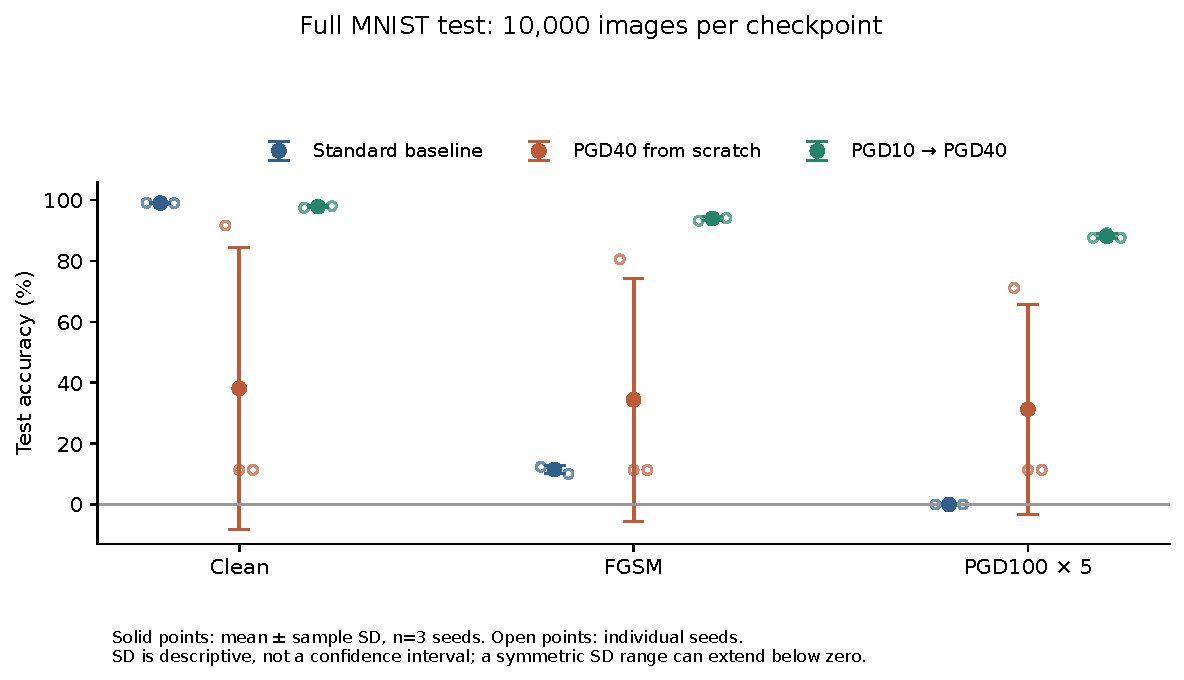
\includegraphics[width=0.99\linewidth]{figures/final_accuracy_comparison.pdf}
\caption{Clean, FGSM and five-restart PGD100 accuracy on the 10,000-image MNIST test set. Error bars indicate sample standard deviations over three independent training seeds, not confidence intervals. All values include collapsed PGD40 runs.}
\label{fig:main}
\end{figure}
\FloatBarrier

\subsection{Per-seed outcomes and comparison with the paper}
\begin{table}[!htbp]
\centering
\caption{Recorded final PGD100$\times$5 results for all three training seeds, including selected validation checkpoint epoch. The CSV records epoch 1 for both low-accuracy direct-PGD40 checkpoints; later-epoch behavior is author-reported because full histories are unavailable.}
\label{tab:seed}
\begin{tabular}{llrrr}
\toprule
Method & Seed & Best epoch & Clean (\%) & PGD (\%) \\
\midrule
Baseline & 0 / 1 / 2 & 10 / 8 / 10 & 99.07 / 99.05 / 98.97 & 0 / 0 / 0 \\
PGD40 & 0 & 10 & 91.66 & 71.15 \\
PGD40 & 1 & 1 & 11.35 & 11.35 \\
PGD40 & 2 & 1 & 11.35 & 11.35 \\
Curriculum & 0 & 10 & 97.50 & 87.62 \\
Curriculum & 1 & 10 & 98.01 & 89.14 \\
Curriculum & 2 & 10 & 98.03 & 87.63 \\
\bottomrule
\end{tabular}
\end{table}

\begin{figure}[!htbp]
\centering
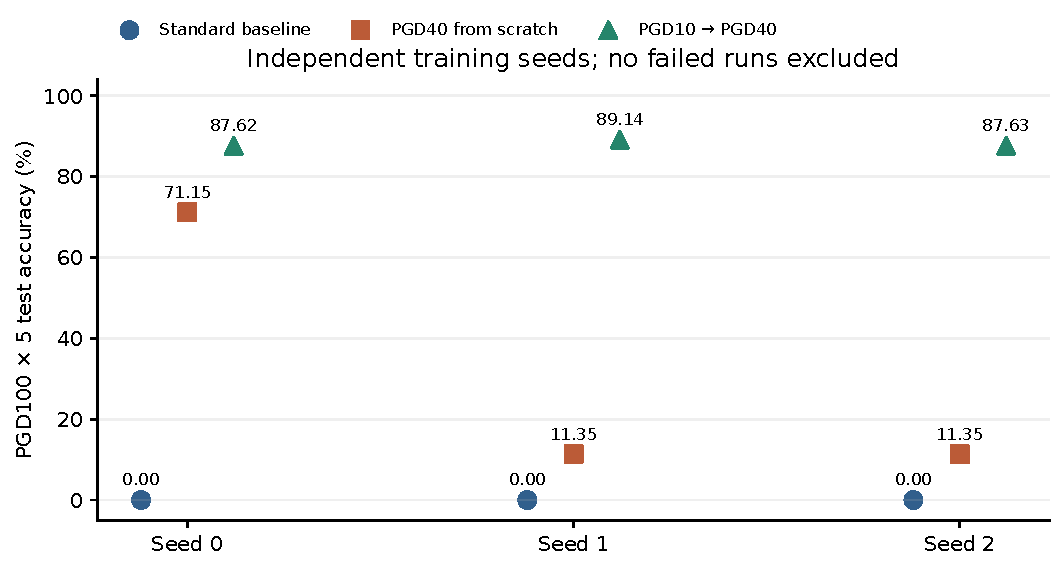
\includegraphics[width=0.9\linewidth]{figures/seed_robustness.pdf}
\caption{Per-seed empirical test robustness with the same PGD100$\times$5 attack. The high variance in direct PGD40 reflects two $11.35\%$ checkpoints and one substantially stronger checkpoint. All recorded seeds are included; the seed axis does not represent training time.}
\label{fig:seeds}
\end{figure}

The original paper's MNIST Table~1 reports $98.8\%$ natural accuracy and $89.3\%$ against white-box PGD100 with \emph{20} random restarts for an adversarially trained, larger-capacity network \citep{madry2018towards}. Our curriculum model achieves $97.85\pm0.30\%$ clean and $88.13\pm0.87\%$ PGD100 with \emph{five} restarts. These are methodologically related outcomes but \textbf{not an apples-to-apples numerical replication} because the network, training schedule, computational budget, restart count, and model-selection protocol differ. We do not assign an original-paper benchmark to our new curriculum schedule.

\begin{table}[!htbp]
\centering
\caption{Original-paper MNIST Table~1 context versus our results. Rows are \emph{not controlled head-to-head comparisons}: architecture, training budget, and PGD restart counts differ. The original row is a reported literature result for a larger adversarially trained model, not a measurement from our experiments.}
\label{tab:paper}
\begin{tabular}{p{0.39\linewidth}cc}
\toprule
Model / evaluation protocol & Clean (\%) & PGD100 (\%) \\
\midrule
Madry et al.\ (2018), PGD100$\times$20 & 98.8 & 89.3 \\
Ours: direct PGD40, PGD100$\times$5 & $38.12\pm46.37$ & $31.28\pm34.53$ \\
Ours: curriculum, PGD100$\times$5 & $97.85\pm0.30$ & $88.13\pm0.87$ \\
\bottomrule
\end{tabular}
\end{table}

\FloatBarrier
\subsection{Author-reported supplementary validation checks}
The authors report attacking curriculum checkpoints on the same 512 validation examples with PGD100 and 20 restarts, and full standard AutoAttack, under the stated $\linf$, $\varepsilon=0.3$ threat model. The current standard AutoAttack implementation combines APGD-CE, targeted APGD-DLR, targeted FAB, and Square Attack \citep{croce2020reliable,autoattack_code}. Table~\ref{tab:val} and Figure~\ref{fig:val} preserve the supplied rounded percentages. Raw attack logs, subset indices, historical package version, and checkpoint files were unavailable, so these are \emph{author-reported values, not independently verified reruns}. We do not report component-subset results without their logs. The reported AutoAttack evaluation is on validation only, not on the 10,000-image test set.

\begin{table}[!htbp]
\centering
\caption{Author-reported robust accuracy (\%) for a stated common subset of 512 validation images; raw logs and indices are unavailable. Means and sample SD are recomputed from the displayed rounded percentages across three training seeds; this is not a test-set result.}
\label{tab:val}
\begin{tabular}{lrrrr}
\toprule
Validation attack & Seed 0 & Seed 1 & Seed 2 & Mean $\pm$ SD \\
\midrule
PGD100$\times$20 & 84.38 & 86.52 & 83.98 & $84.96\pm1.37$ \\
Full AutoAttack & 82.62 & 85.16 & 82.23 & $83.34\pm1.59$ \\
\bottomrule
\end{tabular}
\end{table}

\begin{figure}[!htbp]
\centering
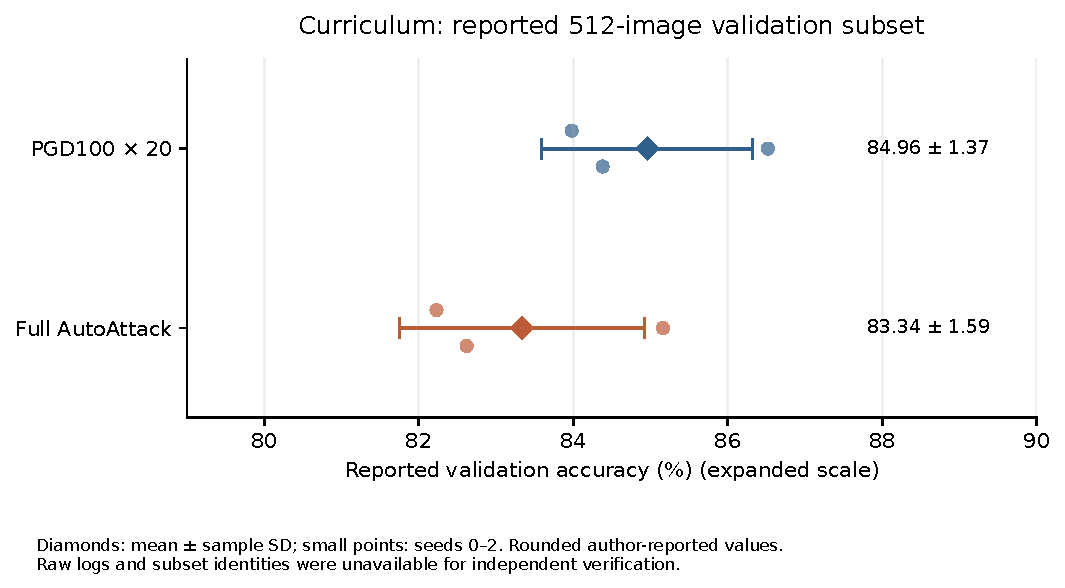
\includegraphics[width=0.9\linewidth]{figures/validation_attack_comparison.pdf}
\caption{Author-reported curriculum robustness for a stated common 512-image validation subset. Raw logs and subset identity remain unverified. The displayed attacks uncover different numbers of failures; these estimates must not be compared directly with the 10,000-image test results because sample and attack differ.}
\label{fig:val}
\end{figure}
\FloatBarrier


\guide{
  \item Report what you measured, without interpretation; interpretation goes in the Discussion.
  \item Put your numbers next to the original paper's numbers. If your setting differs, say so in the caption.
  \item Every number is mean $\pm$ standard deviation over seeds. A single run is not a result.
  \item Recreate the paper's key figure with your own data where possible, so the two can be compared directly.
  \item Every figure needs labelled axes with units, a legend, and a caption that can be understood without the text. Refer to every table and figure in the text.
}

\section{Discussion}
\label{sec:discussion}
\textbf{Does the claim hold?} \emph{Yes, conditionally in our scaled setting.} Standard training attains around $99\%$ clean test accuracy but no correct predictions under our strongest frozen test attack, while the curriculum adversarially trained models retain $88.13\pm0.87\%$. The direct PGD40 condition also demonstrates the mechanism when optimization succeeds (seed 0: $71.15\%$ robust test accuracy), but it is highly unstable under our small network and chosen hyperparameters. Thus our results support the broad adversarial-training claim without establishing universal superiority for every training schedule or initialization.

\textbf{Collapse and optimization sensitivity.} The endpoint CSV records $11.35\%$ accuracy for direct PGD40 seeds 1 and 2. The authors describe failures persisting through ten epochs and report epoch-3 diagnostics with nearly constant logits, predictions of digit 1 on 1,000 validation inputs, and very small early-layer gradients. The diagnostic tensors, prediction counts, and histories were unavailable for this audit, so these observations cannot be independently confirmed from aggregate accuracies alone. Both seeds' best checkpoints were selected at epoch 1, with clean and PGD test accuracy both $11.35\%$. The latter does \emph{not} indicate that a useful classifier withstands PGD: a constant predictor can have similar accuracy with and without perturbations. The observations are consistent with representation/optimization collapse but do not conclusively establish a particular cause such as ``dying ReLU.'' The smaller network, strong attacks from initialization, learning rate, and initialization differences from the original are all plausible contributing factors.

\textbf{Exploratory curriculum.} Motivated by the collapse, we trained PGD10 models for three epochs before continuing with PGD40 for seven more. As described in the execution-provenance subsection, the authors report transferring training state from three PGD10 runs; the repository now also offers direct epoch-dependent scheduling from a fresh run. The original transfer artifacts were not available to test exact equivalence. All three observed curriculum runs trained successfully, with substantially lower between-seed variation in robustness. This exploratory comparison is consistent with the hypothesis that a gentler initial adversary can stabilize early optimization, but three seeds and incomplete execution records do not establish causality or a general failure probability. The authors report choosing the schedule from validation behavior before final testing.

\textbf{Attack validity and limitations.} The author-reported 512-example validation summaries are $84.96\pm1.37\%$ for PGD100 with 20 starts and $83.34\pm1.59\%$ for full standard AutoAttack. Their means are computed from rounded inputs; exact counts would be needed to resolve last-decimal rounding. The authors also report a Square Attack warning and a higher-budget seed-0 check reducing accuracy from approximately $82.62\%$ to $82.42\%$. Without the original logs, the warning, query/restart settings, and this extra result remain unverified. The official implementation warns when Square finds enough additional failures and recommends more iterations/restarts or an adaptive attack \citep{autoattack_code}. This difference is small on 512 images but does \emph{not} eliminate the possibility of gradient masking or stronger adaptive attacks \citep{croce2020reliable}. PGD and AutoAttack numbers are empirical, not certified. AutoAttack was applied to 512 validation examples rather than the full test set, and the full training histories were not attached to this report-generation snapshot, so Figure~\ref{fig:main} summarizes endpoints rather than claiming a complete loss-vs-epoch trajectory.

\textbf{Comparability and further work.} Our network is considerably smaller than the authors' two-convolution, 1024-hidden-unit MNIST model; its training budget is shorter, with different initialization and optimizer settings. This makes direct equality of accuracies uninterpretable, although the \emph{direction} of the clean-versus-robust comparison is meaningful. Three seeds provide limited precision for estimating the failure frequency of direct PGD40. More compute would support capacity and learning-rate ablations, additional seeds, full-test AutoAttack, Square Attack budget sweeps, and publication of complete training curves from saved \texttt{history.csv} logs. The analysis leaves failures in the results instead of selecting only successful runs.


\guide{
  \item Answer directly: does the claim hold in your setting, partially hold, or not hold?
  \item Explain every agreement and disagreement with the original results using the theory from Section~\ref{sec:method} and your deviations from Section~\ref{sec:setup}.
  \item State which conclusions depend on seed, initialization or hyperparameter choices. If the difference between two methods is smaller than the spread over seeds, say so.
  \item A careful, well-explained failure to reproduce is a valid result. An unexplained one is not.
  \item State the limitations of your reproduction and what you would test next with more compute.
}

\section{Conclusion}
\label{sec:conclusion}
On a free-GPU MNIST reproduction, ordinary training produced accurate yet PGD-vulnerable classifiers, whereas adversarial training could yield substantial empirical robustness. Direct PGD40 optimization was unreliable across three seeds in the scaled-down network, while a PGD10$\rightarrow$PGD40 curriculum produced $88.13\pm0.87\%$ robust test accuracy under a frozen 100-step, five-restart PGD evaluation. The main robust-training claim of \citet{madry2018towards} is supported in this restricted setting, with caveats about architectural differences, training stability, and attack-evaluation limits.


\guide{
  \item A short paragraph: what you tested, what you found, and what it means for the paper's claim.
  \item No new results or arguments here.
}

\section*{Contributions}
\label{sec:contrib}
\textbf{Author-reported work and assigned final reviews.} The roles below preserve the contribution account supplied with the project; the audit does not independently verify who performed each activity. Assigned reviews are not represented as completed and must be confirmed by their respective authors before submission.
\begin{itemize}[leftmargin=1.5em]
\item \textbf{Muhammed Emir Baka\c{c} (2368574) --- author-reported completed work:} Ran the Colab training and final model evaluations, verified the nine-model result table, maintained the public GitHub repository, and coordinated reproducibility documentation and report preparation.
\item \textbf{Mehmet Efe \c{C}ak\i r (2201123) --- assigned theory and methodology review:} Check the robust optimization formulation and the FGSM/PGD derivations in Section~\ref{sec:method}; verify that the threat model and implementation description agree with the original paper and referenced source code.
\item \textbf{Sena Sa\u{g}d\i\c{c} (2201275) --- assigned results and manuscript review:} Cross-check all per-seed results, means, and sample standard deviations against the final CSV; verify figure labels and captions; proofread citations, language, and report formatting.
\end{itemize}
The final manuscript should be checked and approved by all three authors after these reviews.

\guide{
  \item Describe concretely what each member did (derivation, implementation, experiments, writing).
  \item Every member is expected to understand the whole project, not only their own part.
}

\section*{Use of AI Tools}
ChatGPT and Codex assisted with experimental planning, code and regression tests, debugging, analysis, figure preparation, and drafting and editing of documentation and this report. The authors report running training and attack evaluations in Colab. The final audit recalculated statistics from the preserved result CSV and checked the available source; it did not rerun the historical GPU experiments or verify missing checkpoints and validation logs. The student authors remain responsible for the analysis, contribution statements, and submitted work.

\section*{Code}
\phantomsection
\label{sec:code}
\url{https://github.com/emirbakac/cmp4509-madry-mnist}


\guide{
  \item Mandatory: link to your group's own public GitHub repository containing the reproduction. A report without it receives 0 points.
  \item The repository needs a README explaining how to run the code.
  \item The notebooks must run top to bottom on a free platform (Colab or Kaggle) and produce the numbers and figures in this report.
}

\bibliographystyle{plainnat}
\bibliography{references}

\guide{
  \item Cite the original paper and every other source you used, including code repositories and blog posts.
  \item Use BibTeX entries from the publisher or the venue, not from search-engine snippets.
}

\end{document}
